\mychapter{4}{Proposed work}
%
% The proposal should address the feasibility of various experiments and point out caveats that might be encountered and how these could be circumvented. Be sure to include positive and negative controls, analysis and interpretation, pitfalls and alternative approaches, and somewhat detailed methods. Prioritize
%

%%%%%%%%%%%%%%%%%%%%%%%%%%%%%%%%%%%%%%%%%%%%%%%%%%%%%%%%%%%%%%%%%%%%%%%%%%%%%%%%%%
%%%%%%%%%%%%%%%%%%%%%%%%%%%%%%%%%%%%%%%%%%%%%%%%%%%%%%%%%%%%%%%%%%%%%%%%%%%%%%%%%%
\section*{Name-face association task}
%%%%%%%%%%%%%%%%%%%%%%%%%%%%%%%%%%%%%%%%%%%%%%%%%%%%%%%%%%%%%%%%%%%%%%%%%%%%%%%%%%
%%%%%%%%%%%%%%%%%%%%%%%%%%%%%%%%%%%%%%%%%%%%%%%%%%%%%%%%%%%%%%%%%%%%%%%%%%%%%%%%%%
%%%%%%%%%%%%%%%%%%%%%%%%%%%%%%%%%%%%%%%%%%%%%%%%%%%%%%%%%%%%%%%%%%%%%%%%%%%%%%%%%%
\subsection*{Background}
%%%%%%%%%%%%%%%%%%%%%%%%%%%%%%%%%%%%%%%%%%%%%%%%%%%%%%%%%%%%%%%%%%%%%%%%%%%%%%%%%%
To investigate the effects of sleep on memory consolidation, I propose creating an audio-visual name-face association task administered with an intervening period of sleep between training and testing phases. Additionally, we will assess whether auditory stimulation of name cues during sleep further promotes memory consolidation. Ultimately, I intend to test the hypothesis that reactivation of task related network dynamics underlie memory consolidation during sleep, and that auditory cues enhance these reactivation effects.

\subsubsection*{Face-name association}
Studies on the neural correlates of face-name association have been explored extensively with fMRI \citep{Sperling2001}. However, while faces are common stimuli in human iEEG studies, a face-name association task has not been published in these subjects, to my knowledge \citep{Quiroga2005, Mormann2015, Zheng2017}. 

Associating names with faces and recalling that association is a pre-requisite for many social interactions. Yet due to the inherent arbitrariness of a names, this is a particularly challenging task; in fact, more difficult than associating faces with other biographical information, such as occupation \citep{McWeeny1987, Rentz2011}. Remembering names is also the greatest complaint in older adults, and likewise has clinical relevance to AD \citep{Vannini2012}. In fMRI, this task has been shown to recruit hippocampus, fusiform gyrus, thalamus, as well as visual, posteromedial, and prefrontal cortices \citep{Sperling2001,Rentz2011}. Importantly, task active brain regions further emphasize the relevance face-name association to AD and sleep as they coincide with the default mode network and hippocampus, which accumulate A$\beta$ and tau preferentially \citep{Raichle2001, Buckner2005a, Pariente2005,Rentz2011, Vannini2012, Mander2015, Mander2016}.

%16 image-text face, name and occupations associations. Free recall.\citep{Rentz2011}. 80 image-text face-name pairs 2.75 sec. 4 encoding runs with 20 face-name pairs presented 3 times. and 4 retrieval trials.\citep{Vannini2012}
\subsubsection*{Stimulus cues during sleep enhance memory}
Despite unconsciousness, sensory stimulation has been shown to evoke neural activity \citep{Sela2016b, Pereira2017, Sharon2017}. These stimuli can also be used to promote sleep brain rhythms and enhance memory as a result \citep{Ngo2013}. Although the stimuli do not reproduce the typical neural processing associated with cognition, they do elicit activity resembling sensory processing \citep{Makov2017e}. Yet despite, the apparent lack of typical cognitive processing, stimulus cues previously associated to task behavior improve the memory specifically for the associated behavior \citep{Rasch2007, Rudoy2009a, Antony2012,Creery2015}.

\subsubsection*{Memory replay}
While there are many reports of replay events during sleep in rodents, evidence is lacking in humans. Early research on replay was generally presented in the context of the hippocampal multi-unit firing patterns, but memories are also coded in distributed cortical networks \citep{Wilson1994, Hoffman2002, Yassa2013, Wilber2017}. Lately, more emphasis has been placed on the interactions between the hippocampus and cortex which are believed underlie memory consolidation, and occur frequently during sleep \citep{Rasch2013, Abel2013}. Specifically, these consolidation processes are thought to involve cortical SWs, thalamic spindles, and hippocampal SWRs \citep{Siapas1998, Molle2006, Maingret2016, Skelin2018}.

A recent human iEEG study provided the first purported evidence of replay in humans \citep{Jiang2017}. In the report, sequences of HG activity that repeatedly occurred during wake were shown to be partially reactivated during sleep. In most subjects, these repetitive sequences were chosen during spontaneous activity, but in three other subjects, sequences were chosen during tasks $-$ a movie (Zoolander) in two subjects and a face-name association task in another. Critically, this study failed to show evidence that memory was improved as a function of the purported replay events, and due to the sparse task data and variability, the cognitive relevance of these sequences is dubious. To conclusively show evidence of replay, it is necessary to show that unique task-relevant activity patterns are reactivated, and that such reactivation improves memory performance on the task. To that end, I have designed an audio-visual name-face association task various trials to solicit reactivation by cuing memory recall in various ways.  

%%%%%%%%%%%%%%%%%%%%%%%%%%%%%%%%%%%%%%%%%%%%%%%%%%%%%%%%%%%%%%%%%%%%%%%%%%%%%%%%%%
\subsection*{Methods}
%%%%%%%%%%%%%%%%%%%%%%%%%%%%%%%%%%%%%%%%%%%%%%%%%%%%%%%%%%%%%%%%%%%%%%%%%%%%%%%%%%
\subsubsection*{Stimuli}
The task I propose involves learning associations between static images of faces audio clips of names. Face stimuli will be drawn from the NimStim database, which features static color images of people taken from above the shoulders and set on a light backdrop. We will use faces expressing one of three emotional affects: happy, neutral, or angry. The face will be set in front of a light backdrop and the images will be centered on computer screen with a black background. Finally, any text will be presented with standard sans-serif font in white.  Names will be drawn from the social security database of names listed by frequency in the US and California. The audio of names will be spoken in a standard American English accent and with a neutral tone.
%and will be either recorded by voice actors or clipped from existing audio - for example on YouTube. 
% (https://www.ssa.gov/oact/babynames/)

\subsubsection*{Training}
During the training phase, subjects will be presented with 120 face-name pairs. Each presentation will be preceded by a white fixation cross on a black background for a  duration of 500 ms. For each stimulus pair, a face will be presented first, and followed 500 ms later by an audio clip of the corresponding name. The face will then remain on display for an additional 500 ms so it is presented for a total of 1000 ms. A screen will follow instructing the subject to imagine a person with that face and name. The end of the trial will be signaled by a beep 1000 ms later and the fixation cross will reappear.

To prevent anticipatory effects, the timing of each portion of the task could instead be variable. Additionally, to ensure subjects cease imagination at the end of the trial, a distractor stimulus could be administered during the fixation period; for example, the fixation cross could be presented on a background of continuously changing white noise and/or accompanied by white noise audio. 

\subsubsection*{Test}
Test phases will be administered immediately following training (pre-test) and again after sleep (post-test). During this phase, a face will be presented for up to 1500 ms, and subject may respond vocally at any time by uttering a name into a microphone. For the pre-test phase, the trial will always end with the original audio clip of the corresponding name, but no feedback will be provided during the post-test. Following feedback will be a fixation period like training period.

This task will be facilitated with voice recognition of names implemented by integrating an existing api such as Google voice to evaluate subject input during each test trial and determine if it is correct. However, to ensure quality, the subject responses will also be manually reviewed after administration. During the pre-test, each face will be presented at least two times in random order; however, a face will be presented up to five times or until it is correctly identified at least once - as determined by voice recognition.

\subsubsection*{Name cued imagination}
Following the pre/post-test sessions, will be a name cued imagination phase. In this session, audio clips of names will be presented followed by a blank screen, during which subjects are supposed to imagine the corresponding person. The trial will end identically to the training phase, i.e. signaled and followed by a fixation period.

\subsubsection*{Sleep}
Before the post-test session, subjects will sleep for at least one hour. Prior to them sleeping, one half of the names will be selected to be played during sleep; the subset will be chosen pseudo-randomly ensuring that both halves are matched for gender and emotional affect. Volume will be set at a non-disruptive level below that of quiet conversation so that the patient will not be woken. Furthermore, a system could be developed to monitor low-frequency power and only present stimuli during slow wave sleep .

\subsubsection*{Subjects}
Although this task was designed for patients implanted with iEEG to probe fast network dynamics supporting to memory consolidation during sleep, it need not be limited to this population. With some modifications it can be implemented for other populations to be studied using EEG and/or MRI. In fact, this task is used frequently to study effects of age and dementia on memory; for example, performance on such a task is predictive of amyloid burden \citep{Rentz2011, Vannini2012}.

\subsubsection*{Equipment}
This task will be designed to run on the Lin lab computer used for task administration. It will require two 3.5 mm male-male auxiliary cords, a male-female/female auxiliary splitter, and speakers. The audio from the task will be output through the splitter cable and routed to the speakers and to the DC input box so that the audio signal is recorded simultaneously with neural data aquisition. This audio recording will allow for the task presentation to be aligned with neural recordings for analysis. Additionally, an application on the computer will record task data and microphone data as separate channels so the microphone data can also be aligned to the neural recordings.

%%%%%%%%%%%%%%%%%%%%%%%%%%%%%%%%%%%%%%%%%%%%%%%%%%%%%%%%%%%%%%%%%%%%%%%%%%%%%%%%%%
\subsection*{Analyses}
%%%%%%%%%%%%%%%%%%%%%%%%%%%%%%%%%%%%%%%%%%%%%%%%%%%%%%%%%%%%%%%%%%%%%%%%%%%%%%%%%%
The goal of this task is to study the effect of sleep on memory consolidation and determine if the reactivation of neural dynamics supports this consolidation. Memory consolidation will be assessed behaviorally by post-test vs pre-test task performance on the basis of correct identification and reaction time. We expect correct identification to increase and reaction time to decrease reflecting sleep related memory consolidation effects. Furthermore, we expect this effect to be greater for the subset of names which were played during sleep.

To assess network reactivation, the first step will be establishing a method to derive network dynamics. Previous work purportedly showed evidence of replay using sequences of peaks in high gamma (HG) power; basically, HG power will be determined using wavelets, peaks will be detected as local maxima in power, and the sequence of these peaks will be compared across trials $-$ since method has been published, it will be a good starting point. Additionally, this method could be extended to other frequency bands of interest. Alternatively, the method I developed for detecting traveling waves could be used to characterize network activity.

Task network dynamics will be determined for each distinct task interval of each trial. More specifically, faces, are presented in three distinct contexts (F1) without and (F2[N1]) with a name during training and (F3) during testing; furthermore, reactivation of neural representations of the faces is cued for imagination during (F4) training and in the (F5) name cued imagination session. Similarly, names are presented three ways: with faces (N1[F2]) during training and as cues (N2) for imagination trials as well as (N3) during sleep; additionally, names are cued to be (N4) recalled and (N5) spoken during testing. To first characterize general face and name networks, F1 to F5 and N1 to N5 will be combined. These context can be separated or grouped in various ways to determine how the networks change based on context.

For instance, to determine how perceived and imagined, i.e. reactivated, representations differ, F1 to F3 will be contrasted with F4 $\&$ F5. Similarly, to evaluate how name processing differs during sleep, N1 $\&$ N2 will be contrasted to N3. More importantly, to assess the extent to which face representations are replayed following cues during sleep, the F4$\&$F5 network will be compared to N3 trials. We expect that N3 trials will vary in their similarity to N1 $\&$ N2 and F4 $\&$ F5, but high correspondence with F4 $\&$ F5 (indicative of face replay) will entail high correspondence with N1 $\&$ N2 (indicating name processing); furthermore, high N3 - F4$\&$F5 correspondence should predict improved performance on the corresponding face-name association. To seek evidence of spontaneous replay, networks will be derived from intervals of sleep without cues, and will be compared to F4 $\&$ F5. We hypothesize that windows with high correspondence will also feature SW, spindle, SWR, or combinations of these waves.

%We hypothesize that correct trials will have a higher inter-trial network similarity and sequences with shorter lag time.
%Various post-hoc constrasts can
%but its rich design will enables various effects to be finely parsed.
%Hypothesize task response will involve activity in near the superior lateral temporal lobe during name stimuli presentation. Then during face stimuli presentation, occipital lobe and fusiform gyrus activity will increase. We expect each of these activities to exhibit functional connectivity to the hippocampus and frontal lobe during imagined reactivation and.

%%%%%%%%%%%%%%%%%%%%%%%%%%%%%%%%%%%%%%%%%%%%%%%%%%%%%%%%%%%%%%%%%%%%%%%%%%%%%%%%%%
\subsection*{Discussion}
%%%%%%%%%%%%%%%%%%%%%%%%%%%%%%%%%%%%%%%%%%%%%%%%%%%%%%%%%%%%%%%%%%%%%%%%%%%%%%%%%%
While face-name association tasks have been widely used in fMRI studies, they have not been adopted by the iEEG community; moreover, given the extensive literature on single unit activity in the MTL evoked by faces, such a task offers an opportunity to study how these responses might be formed for novel face-name pairs \citep{Quiroga2005, Mormann2015, Viskontas2016}. Similarly, memory enhancement from stimulus cuing during sleep has been explored in scalp EEG and fMRI, but not in iEEG; notably, this task may be able to answer whether memory reactivation underlies this memory enhancement \citep{Rasch2007a,Antony2012,Creery2015, Makov2017e}. While, these task designs will be novel contributions to iEEG literature, more importantly, they are tools we will use to evaluate whether replay enhances memory consolidation during sleep in humans. Although replay was purportedly demonstrated in humans last year, this study had major weaknesses. Crucially, the report did not utilize consistent task behavior, and likewise replay-like events could not be related to memory and only vaguely to cognition \citep{Jiang2017}. This study used cortical HG as evidence of replay; however, providing evidence of replay with single unit activity the MTL is now possible at UCI, and would greatly strengthen evidence of replay. 

Another strength of the task is its rich design which would enable various post-hoc analyses; for instance, differences in neural representation and/or memory performance related to sex or emotional affect could be explore. This task is also easily extensible for future studies; for example, to further examine the effect of emotion on memory consolidation, names could be spoken with expressive voices. Another potential avenue to explore are richer stimuli biographies beyond just their name, such as occupation or interpersonal details about relationships between the hypothetical people represented by the stimuli \citep{Rentz2011}. 

Due to stimulus cuing during sleep, it is possible, this study will need further IRB approval, which could delay its implementation; however, this presents little risk to patients besides potential awakenings, and that risk will be mitigated by volume control and possibly the implementation of a closed-loop system limiting stimulus presentation to SWS, when they are unlikely to awaken. A potential risk of this proposal is that the Jiang study did mention a single patient participating in a face-name association task, which may suggest that Dr. Halgren's group is actively administering this task $-$ potentially for a follow up study on replay. It is also possible, that we will not find evidence of replay in this task, but because of the stronger experimental design of this task, the negative result would call into question \citep{Jiang2017}. Moreover, due to the sparsity of intracranial literature on face-name association, just reporting the associated neural processing and effects of sleep on memory would be a novel contributions. Overall, I think the strengths of this study far outweigh the potential short-comings.

%%%%%%%%%%%%%%%%%%%%%%%%%%%%%%%%%%%%%%%%%%%%%%%%%%%%%%%%%%%%%%%%%%%%%%%%%%%%%%%%%%
%%%%%%%%%%%%%%%%%%%%%%%%%%%%%%%%%%%%%%%%%%%%%%%%%%%%%%%%%%%%%%%%%%%%%%%%%%%%%%%%%%
\section*{Evaluating Glymphatic Activity in Humans}
%%%%%%%%%%%%%%%%%%%%%%%%%%%%%%%%%%%%%%%%%%%%%%%%%%%%%%%%%%%%%%%%%%%%%%%%%%%%%%%%%%
%%%%%%%%%%%%%%%%%%%%%%%%%%%%%%%%%%%%%%%%%%%%%%%%%%%%%%%%%%%%%%%%%%%%%%%%%%%%%%%%%%
\subsection*{Background}
Essentially, glymphatic activity refers to the flux of CSF into, out of, and within brain parenchyma. As discussed in the introduction, the glymphatic system is activated during SWS as it flushes CSF through the brain parenchyma to remove metabolites accumulated from the processes necessary to maintain wakefulness. Thus, by preventing, the accumulation of toxic proteins like A$\beta$. Glymphatic clearance during sleep may play a critical protective role, and likewise, its disruption could be an early mechanistic factor in the development of Alzheimer's pathology as well as other diseases. However, due to a lack of methods suitable for imaging glymphatic activity which also satisfy the paramount ethical considerations for studying human subjects, there has been little evidence of this activity in humans. In this section I propose a extending phase contrast magnetic resonance imaging (PCMRI) to study glymphatic activity in humans and its relationship with age and dementia.
%I will discuss a few MRI sequences that measure fluid movement and how they might be adapted in order to image glymphatic activity. In addition, I will consider the complexities of the system and inherent limitations of MRI technology, and suggest strategies to address these issues. 

Nearly all studies of the glymphatic system to date have involved time resolved imaging of an exogenous tracer, and shown that tracer distribution in the brain increases with time, especially during sleep \citep{Iliff2012,Iliff2014,Xie,Peng2016}. However, most of these methods cannot be implemented in humans because the imaging technique, i.e. 2-photon microscopy, is too invasive, and the tracers are toxic. One exceptional method was developed using contrast-agent MRI based on the element gadolinium (Gd) $-$ essentially a paramagentic tracer \citep{Iliff2013,Yang2013}. While, Gd-based contrast-agents are sometimes clinically indicated for a small subset of patients $-$ for example, in the diagnosis of stroke or brain tumor $-$ gadolinium is a heavy metal, and likewise toxic, so to reduce it’s toxicity, clinical Gd-based contrast agents are administered as a compound with a chelating agent to cage the metal, thus preventing it from interacting with biological tissue. Although atomic gadolinium may freely cross the blood-brain-barrier, the chelating agents are too large to pass. So while, non-chelated gadolinium has been used to image the glymphatic system in rodents, clinical Gd-based contrast agents are not suitable for that purpose \citep{Iliff2013,Yang2013,Lee2015}. Nevertheless, these clinical contrast agents have been successfully applied to imaging the cerebral lymphatic vessels located near the superior saggital sinus in non-human primates and humans \citep{Absinta2017}. It should also be noted that even chelated Gd-compounds, despite FDA approval, are known to accumulate in the brain and the long-term consequences of this are not well understood.

\subsection*{Methods}
\subsubsection*{Subjects}
I will seek participation from a large cohort of subjects who are already participating in MRI studies and cognitive evaluations through an ongoing collaboration with UCI's Alzheimer's Disease Research Center (ADRC) and Dr. Yassa's project, "High-Resolution Neuroimaging Biomarkers for Preclinical Alzheimer’s Disease." Although these subjects do not have clinical indications of AD they are ages 65-85, well within the age range at risk for development of AD; likewise, the goal of Dr. Yassa's project is to identify biomarkers of brain dysfunction in the preclinical stages of AD. Based on studies in rodents, disruption in glymphatic clearance is a strong candidate for such preclinical dysfunction. From another of Dr. Yassa's ongoing projects, "Biomarkers of Alzheimer’s Disease in Adults with Down Syndrome", we will attempt to recruit individuals with Down Syndrome, a another population at risk for the development of AD. Additionally, I will try to forge new collaborations with UCI's brand new Sleep and Circadian Neuroscience (SCN) Center, directed by Dr. Ruth Benca. Individuals participating in research here may have a sleep-disorder, thus comprising a third population at risk for developing AD. Finally, I will recruit young, healthy subjects from UCI's campus. 

\subsubsection*{MRI}
%It is clear that existing methods for imaging the glymphatic system are incompatible with the critical ethical and safety concerns inherent to human studies. For this purpose, 
To image the glymphatic system in humans, a technique must be minimally invasive; have high enough spatial resolution and contrast to distinguish small subarchnoid and paravascular spaces; and the ability to measure changes caused by flow. I think that MRI is currently the best suited technology for this purpose: it is minimally invasive, capable of imaging the entire brain with high ($\sim$.5 mm) resolution fairly rapidly ($\sim$1-10 s), and has an excellent material and movement contrast that can be tuned for particular applications.

MRI scanners utilize a phenomenon called nuclear magnetic resonance (NMR). Basically, NMR manipulates a quantum property of atomic nuclei, called spin, with pulses of precisely tuned electromagnetic fields to align the nuclear spins in a way that encodes information about time and space, and can be used to infer the chemical composition of a material. Atomic nuclei with non-zero spins placed within a magnetic field, called B$_0$, will rotate about an axis parallel to B$_0$ with a frequency proportional to B$_0$'s strength. The frequency of this rotation is determined by the atomic nucleus, typically hydrogen $-$ also referred to as a proton $-$ and it's chemical environment. While all nuclei rotate about this axis defined by B$_0$, each proton occupies one of two possible energy states which determines the direction of its spin: (1) in the low-energy state spin is oriented in the same direction as B$_0$, while (2) in the high energy state spin points in the opposite direction. The low- and high-energy states are called parallel and anti-parallel, respectively, and the natural proportion of spins in these states, called its thermodynamic equilibrium, is related to the sample's composition and temperature. This equilibrium can be perturbed with a burst of electromagnetic radiation, referred to as B$_1$, which is absorbed by some atomic nuclei, thus increasing its energy state. However, the excitation, must be tuned to the resonant frequency of the nuclei, which is identical to its frequency of rotation due to B$_0$, and called the Larmor frequency. For MRI Larmor frequencies occupy the radio frequencies of the electromagnetic spectrum. Following excitation, protons will lose energy through microscopic interactions with its environment, and macroscopically, this is observed as an exponential decay in the sample's energy back to its thermodynamic equilibrium. Importantly, the rate of this decay depends on the properties of the sample, i.e. the microscopic environmental factors that cause spins to return to ground-state $-$ this variable relaxation is the reason why MRI can achieve such spectacular material contrast.

If the sample were exposed to a completely homogeneous B$_0$ and B$_1$, the signal would indicate the relaxation of the sample as a whole, making it impossible to resolve the spatial heterogeneity in the sample. However, the specificity of the Larmor frequency can be leveraged to acquire signals from specific regions of space by using a B$_0$ that varies over space, called a gradient magnetic field, which in turn varies the larmor frequencies over space. In a process known as slice selection, B$_0$ is varied in the z-direction (parallel to the magnetic bore). Then the sample can be excited with a band-limited radio pulse carrying only the frequencies corresponding to the Larmor frequencies in a particular "slice" perpendicular to the z-axis. Additionally, the B$_0$ gradient can be varied along the x and y directions to encode spin frequency and phase, thus enabling small volumes of the sample, or voxels, to be individually resolved. Repeating this technique for many slices, a full 3-dimensional image can be constructed for a sample. However, there are many parameters that can be cleverly manipulated to produce images with specific information encoded \citep{Huettel}.

\subsubsection{Phase contrast MRI}
One way MRI might be used to image the glymphatic activity is to measure flow with phase-contrast MRI (PCMRI) \citep{Hahn1960, Moran1982}. Basically this method uses a gradient magnetic field to encode velocity of protons with phase $-$ essentially using protons as an endogenous tracer. A gradient magnetic field changes field strength relative to B$_0$, thus increasing or decreasing the Larmor frequencies, and likewise shifting the phases of the spins. The amount of phase shift due to the gradient depends on the strength, $G_x$, and duration, $t$, of the field experienced by a proton. 
$$\phi =\gamma x_{0}\int _{0}^{t}G_{x}(\tau )d\tau +\gamma v_{x}\int _{0}^{t}G_{x}(\tau )\tau d\tau +\gamma {\frac {a_{x}}{2}}\int _{0}^{t}G_{x}(\tau )\tau ^{2}d\tau +\ldots,$$
where $\gamma$ is the gyromagnetic ratio \citep{Huettel}. If we assume the starting location and velocity is the primary determinants of phase, we can neglect higher order terms and replace the gradient moments (integrals) with M and simplify this as,
$$\phi =\gamma (x_{0}M_{0}+v_{x}M_{1}).$$ 
From these equations we notice that, if a proton moves along the gradient with velocity, $v_x$, it will experience gradually increasing field strength accompanied by an increasing Larmor frequency, and as a result, its phase will advance relative to stationary protons in its initial starting point, but will be lagged relative to stationary protons at its new location. If the gradient is then reversed and applied for the same duration, the phase shift of all stationary protons will cancel. Although the phase of moving protons would also be reversed by the gradient, it will retain a phase-shift proportional to its velocity, 
$$v = \dfrac{v_{enc}}{\pi}\Delta\phi.$$

\begin{figure}
  \centering
  \includegraphics[scale = .5]{Figures/Lotz_2002_Cancelrad.jpg}
    \caption{Effect of bipolar gradient on stationary and moving protons\citep{Lotz2002a}}
  \label{fig:cnclphi}
\end{figure}

Since this technique relies on phase which can only vary by $360\deg = 2\pi$, a parameter called, $v_{enc}$, determines it's the dynamic range and signal-to-noise ratio,

$$SNR_{v}={\frac {\pi }{\sqrt {2}}}{\frac {v}{v_{enc}}}SNR.$$

Lower $v_{enc}$ will decrease the dynamic range, but also improve the signal for lower velocity activity \citep{Lotz2002a}.

\begin{figure}
  \centering
  \includegraphics[scale = 1]{Figures/PCMRIseq_Turski_2016.jpg}
    \caption{Phase contrast pulse sequence diagram \citep{Turski}}
  \label{fig:pcseq}
\end{figure}


%Flux of CSF can be measured directly by measuring the directed movement of protons or more indirectly by measuring tissue permeability with directed diffusion. Additionally, the overall behavior of CSF fluid dynamics can be characterized by measuring the in-/out-flow, and volume of CSF compartments.

\subsection*{Analysis}
Given that glymphatic activity dramatically increases during sleep, our initial proof-of-concept PCMRI will test the hypothesis that CSF flow through brain parenchyma increases during slow wave sleep relative to wake. The most straightforward way of testing this would be to simply acquire sufficiently many PCMRI scans in both conditions, and compute confidence intervals to show that velocity distributions of parenchymal voxels are significantly greater during sleep. However, we hope to leverage the directional and spatial resolution of PCMRI to show more specific flow changes. Using a T2 image, we will segment subarachnoid and large paravascular spaces, and likewise arteries and veins will be segmented with magnetic resonance angiography and venography. Then with these segmentations, we will more specifically test the hypothesis that flow increases will be greatest near vessels, flowing away from para-arterial space into the parenchyma and from the parenchyma into paravenous space.

It is known that CSF flow is modulated by physiological rhythms such as the cardiac and respiratory cycles, and this modulation will introduce more variability in the flow distributions. However, by simultaneously monitoring this physiology, we can retrospectively align flow measurements to when they were acquired with respect to the physiological rhythm, and constrain the statistical comparisons to commensurate portions of these cycles. So for instance, many samples of flow in a particular PVS voxel can be acquired during wake and sleep, aligned to the cardiac cycle, and then PVS flow measurements acquired during the peak systole can be statistically tested for conditional differences during wake vs sleep.

Currently, we have only acquired a single 2D, 3-directional PCMRI scan with 60 time points, but this initial data is encouraging. The voxelwise standard deviation in fig \ref{fig:sdflow} shows that parenchyma has relatively consistent flow, and the median flow \ref{fig:mdflow} shows there is a particular directionality of the flow. Surely, future scans with more time points, greater spatial coverage, and co-registered csf, angiogram, and venograms will help clarify these images.
%The image was acquired with $v_{enc} = 4$, about two orders of magnitude slower than blood flow in primary vessels.  

\begin{figure}
  \centering
  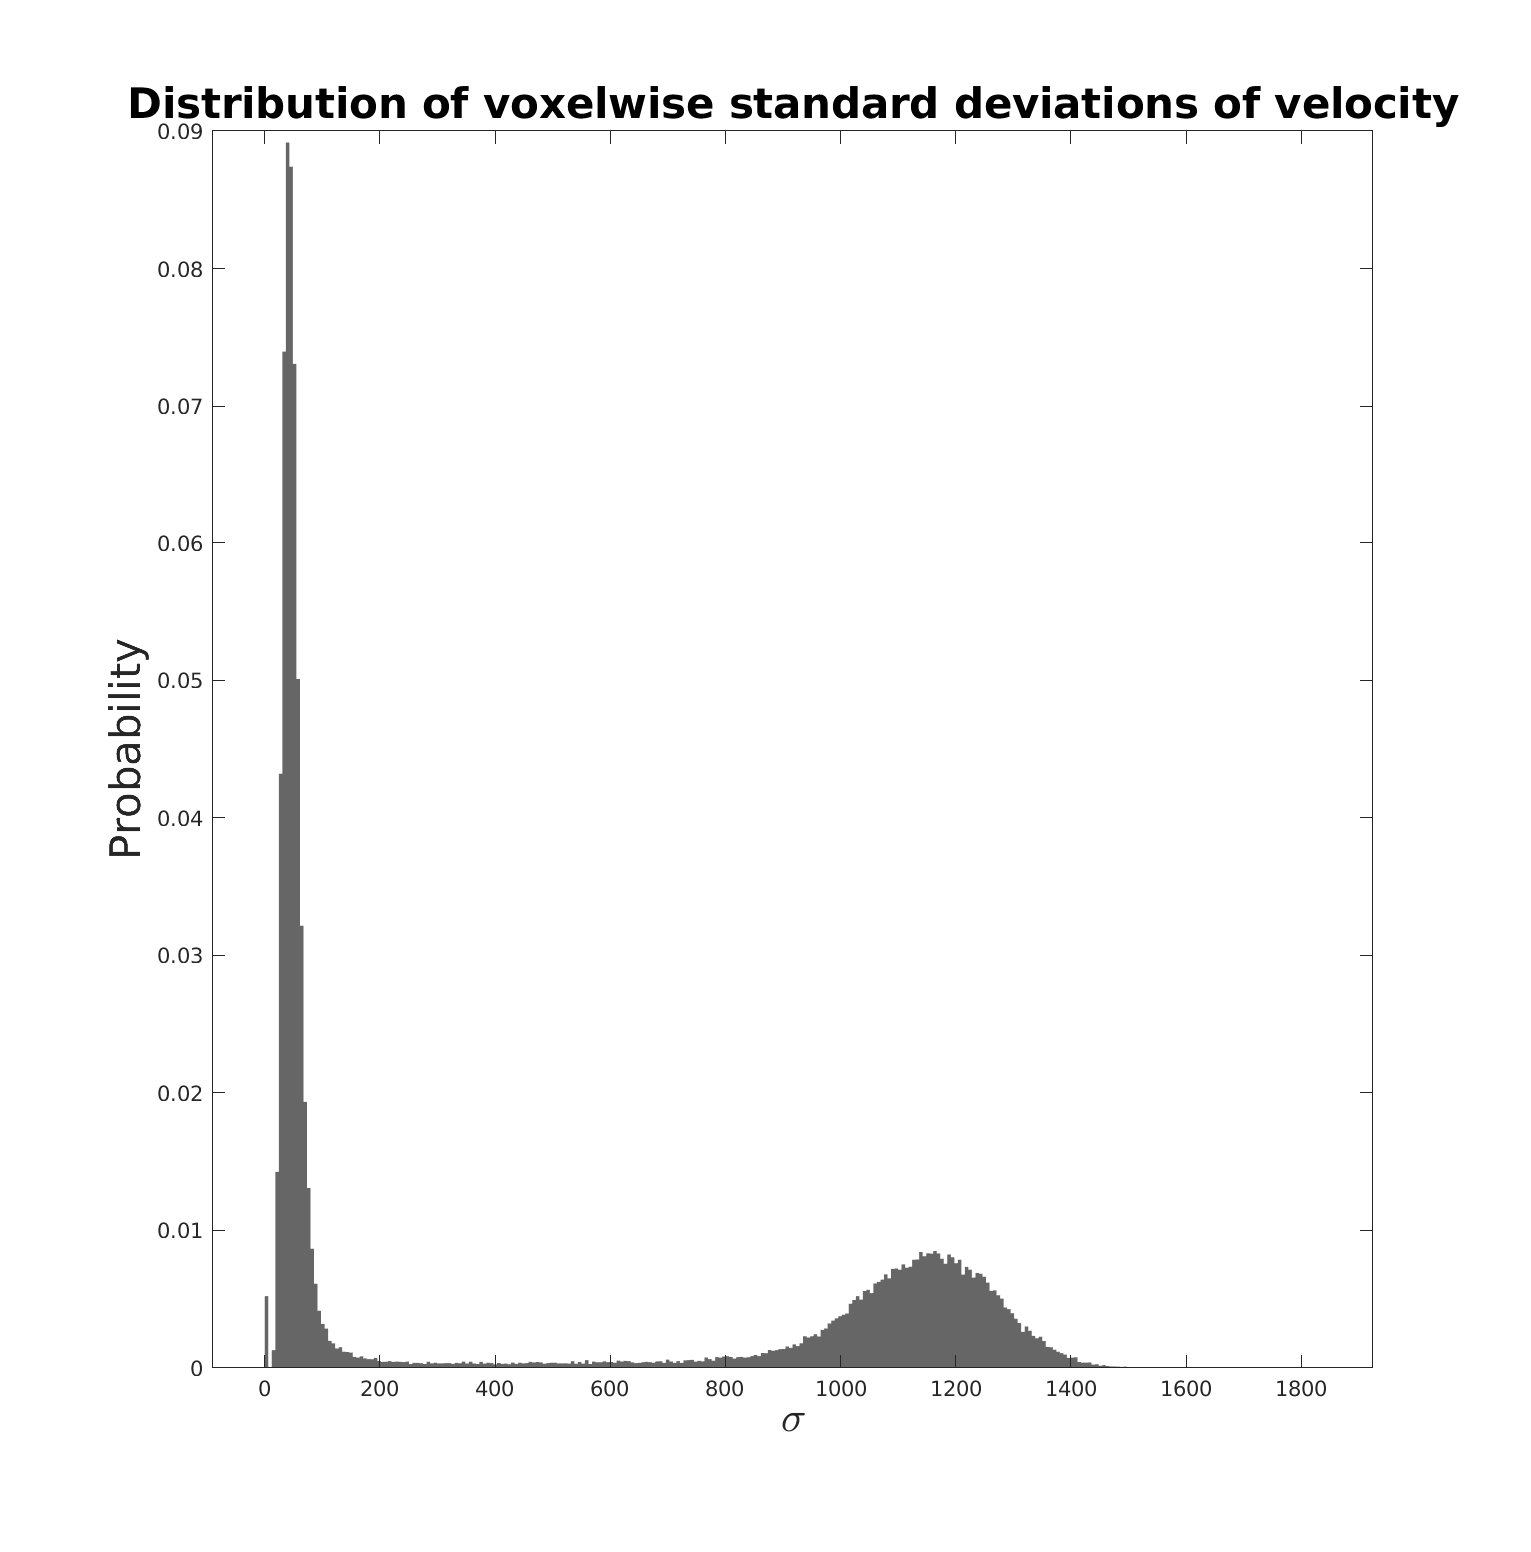
\includegraphics[scale = .45]{Figures/hist_vxl_sd_venc4.eps}
    \caption{Histogram of voxelwise standard deviation of overtime and three phase gradient directions.}
  \label{fig:sdhist}
\end{figure}

\begin{figure}
  \centering
  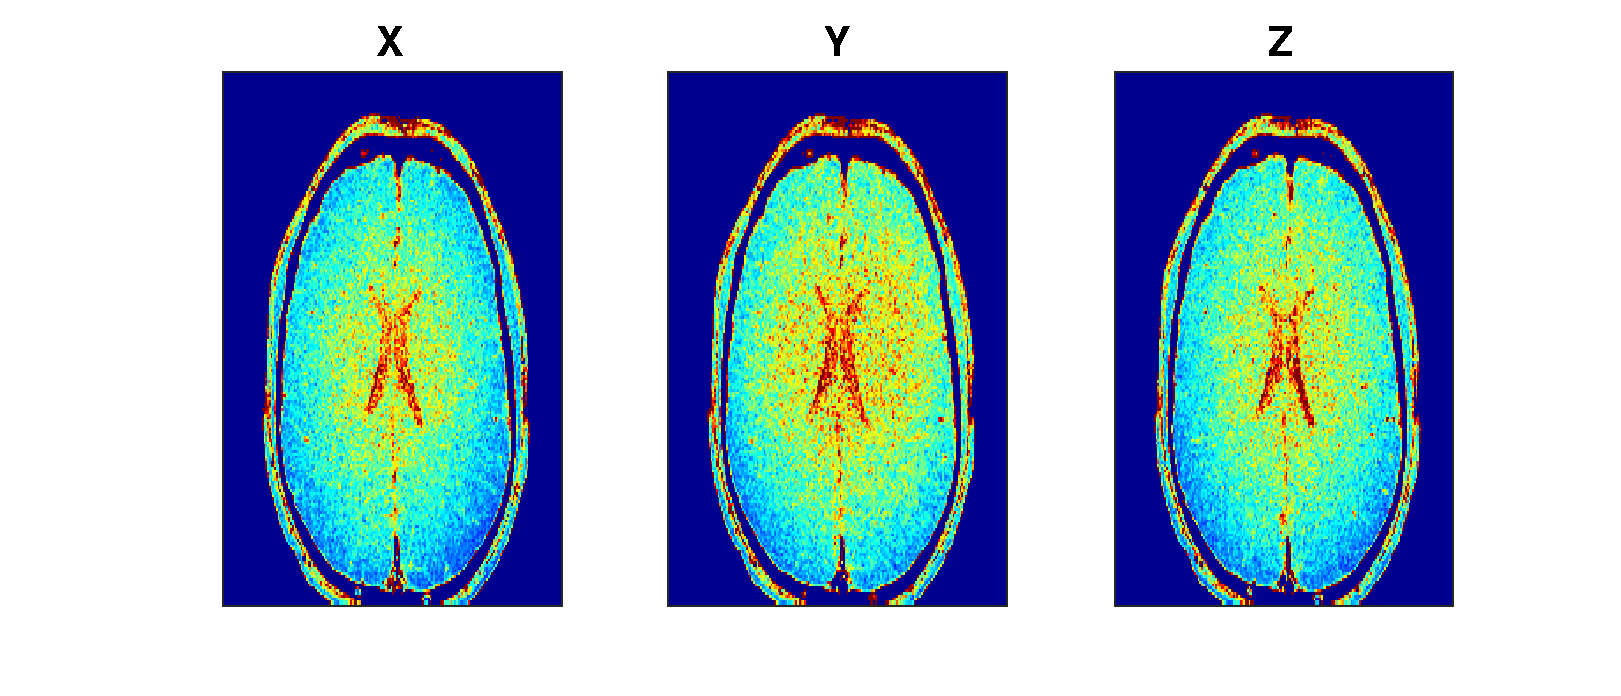
\includegraphics[scale = .6]{Figures/vxl_sd200_venc4.eps}
    \caption{Voxelwise standard deviation for x, y, and z phase gradient directions. \\ Note: voxels with $\sigma > 200$ were supressed.}
  \label{fig:sdflow}
\end{figure}

\begin{figure}
  \centering
  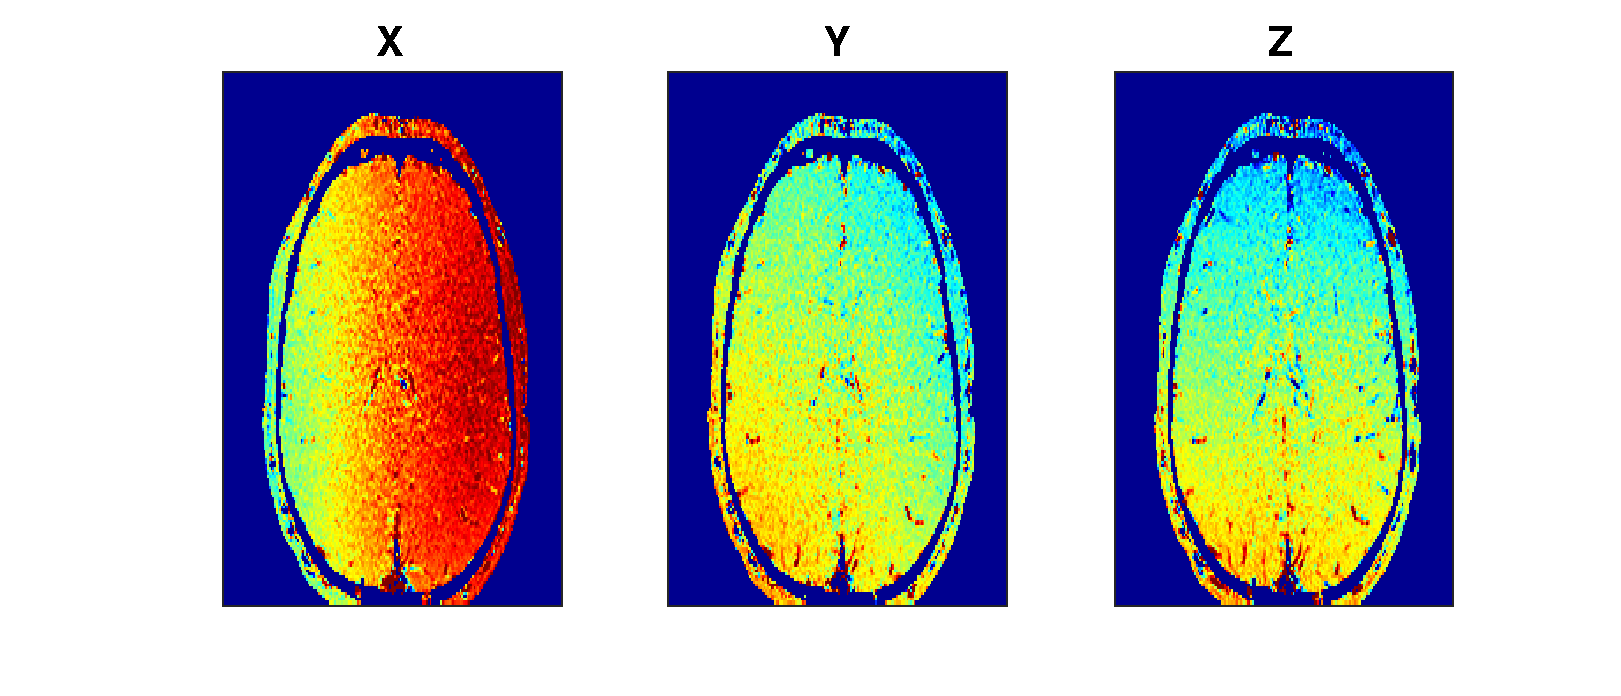
\includegraphics[scale = .6]{Figures/vxl_md150_venc4.eps}
    \caption{Voxelwise median for x, y, and z velocities. \\ Note: voxels with $\sigma > 200$ were supressed.}
  \label{fig:mdflow}
\end{figure}

Following a successful proof-of-concept study, we week seek a collaborator at UCI to help validate this technique with 2-photon microscopy tracer studies in rats. Following a successful validation, we can begin implementing the technique to study glymphatic clearance in healthy controls and subjects at risk for Alzheimer's. Briefly, we hypothesize that CSF flow will generally be both slower and less directed as a function age and other AD risk factors; additionally, we expect sleep will have a diminshed effect on glymphatic clearance in these groups. 

% **Dimensionality reduction techniques**

\subsection*{Discussion}
%At the core of these analyses is properly constraining statistical comparisons of flow measurement by condition, tissue property, and physiological rhythm. 
% Importance
Another potential MRI method to study the glymphatic system involves MR spectroscopy (MRS). This method is a comparable to previous tracer methods, but rather than imaging the distribution of foreign substances, it measures the distribution of endogenous substances over time. Although nothing has been published using this method, it is currently under active development by Jeffrey Illiff and colleagues. Their method involves collecting MRS data overtime to quantify dynamic changes in the distribution of lactate. The choice of lactate was made on the basis of previous studies showing that it accumulates in the interstitial spaces during waking periods, and decreases during sleep as a result of glymphatic clearance. According to Illiff, preliminary results look good, so this may well be the first non-invasive method to image glymphatic activity. However, there are a few potential shortcomings of this method: (1) MRS has a minimum resolution of 1cm3, and (2) it will be sensitive to the natural distribution of lactate in the brain. Studies suggest that lactate is a measure of aerobic glycolysis, or the metabolism of glucose without oxidative phosphorylation despite having sufficient oxygen, and further that this process occurs differentially across the brain, being particularly high in regions involved in the default mode network such as prefrontal cortex, precuneus, and lateral temporal gyrus, but quite low in medial temporal lobe and cerebellar cortex. Therefore, an MRS method based on lactate may be biased, over/understating glymphatic clearance in regions with high/low aerobic glycolysis. In contrast, a PCMRI approach would not have such systematic biases; however, it may be affected by higher noise in areas with lower proton density.

The greatest potential pitfall for this project lacking sufficient resolution and precision of flow measurements to image glymphatic flux. Preliminary data suggests that our 3T MRI can sufficiently resolve various CSF compartments such as the ventricles, subarachnoid space, and pia mater; however, there are only few instances of the PVS surrounding arterioles in deep portions of the brain. Nevertheless, in the glymphatic literature, the subarachnoid space near penetrating vessels are the first regions to show changes in tracer concentration and have the strongest signal, and based on T2 imaging, we can easily image these areas as well as smaller penetrating vessels surround by pia and lining the brains sulci. Furthermore, the initial PCMRI scan seems to indicate that flow in parenchyma can be measured directly, so imaging fine PVS structure may not be necessary. Additionally, the measures of flux must be precise enough to overcome the inherent noise associated with acquiring MRI, but the modest standard deviations in out pilot data seem to indicate good signal. Voxel averaging and variance, movement artifacts, field inhomogeneities, low velocity,


%%%%%%%%%%%%%%%%%%%%%%%%%%%%%%%%%%%%%%%%%%%%%%%%%%%%%%%%%%%%%%%%%%%%%%%%%%%%%%%%%%
%%%%%%%%%%%%%%%%%%%%%%%%%%%%%%%%%%%%%%%%%%%%%%%%%%%%%%%%%%%%%%%%%%%%%%%%%%%%%%%%%%
% TRASH
%%%%%%%%%%%%%%%%%%%%%%%%%%%%%%%%%%%%%%%%%%%%%%%%%%%%%%%%%%%%%%%%%%%%%%%%%%%%%%%%%%
%%%%%%%%%%%%%%%%%%%%%%%%%%%%%%%%%%%%%%%%%%%%%%%%%%%%%%%%%%%%%%%%%%%%%%%%%%%%%%%%%%
%A successful execution would enhance our basic model for how brain rhythms are coordinated in space and how this coordination supports memory. Additionally, we evidence of glymphatic clearance.
%\subsection*{Audiovisual learning}
% Ears. The conical shape of the ear helps to focus air pressure waves onto the eardrum. These vibrations in turn displace a system of three bone -- the malleus, incus, and stapes -- which has the effect of amplifying this signal concentrating this force onto the smaller area of the stapes which beats against the fluid filled chamber of the cochlea. The vibrations of the cochlear fluid propagate through its spiral shape which helps to separate the sound into its frequency components: low frequencies are able to travel the entire length of the spiral, whereas higher frequencies travel shorter distances. Hair cells are located along this chamber, and the vibration of these hairs is finally transduces the original mechanical signal into action potentials which are carried to the brain stem by the auditory nerve. [Brain stem pathway]
%
%Eventually, these signals reach the auditory cortex, where the sounds are believed to be perceived as tones of various frequencies. This sort of fourier sound representation then propagates to other areas to endow the stimulus with more complex perceptions; like the visual system, there are believed to be dorsal and ventral processing streams related to the perception of where and what the stimulus is, respectively.

%%% Local Variables: ***
%%% mode: latex ***
%%% TeX-master: "thesis.tex" ***
%%% End: ***
